% Template for PLoS
% Version 1.0 January 2009
%
% To compile to pdf, run:
% latex plos.template
% bibtex plos.template
% latex plos.template
% latex plos.template
% dvipdf plos.template

\documentclass[10pt]{article}

% amsmath package, useful for mathematical formulas
\usepackage{amsmath}
% amssymb package, useful for mathematical symbols
\usepackage{amssymb}
\usepackage{url}
% graphicx package, useful for including eps and pdf graphics
% include graphics with the command \includegraphics
\usepackage{graphicx}

% cite package, to clean up citations in the main text. Do not remove.
\usepackage{cite}

\usepackage{color} 

% Use doublespacing - comment out for single spacing
%\usepackage{setspace} 
%\doublespacing


% Text layout
\topmargin 0.0cm
\oddsidemargin 0.5cm
\evensidemargin 0.5cm
\textwidth 16cm 
\textheight 21cm

% Bold the 'Figure #' in the caption and separate it with a period
% Captions will be left justified
\usepackage[labelfont=bf,labelsep=period,justification=raggedright]{caption}

% Use the PLoS provided bibtex style
\bibliographystyle{plos2009}

% Remove brackets from numbering in List of References
\makeatletter
\renewcommand{\@biblabel}[1]{\quad#1.}
\makeatother


% Leave date blank
\date{}

\pagestyle{myheadings}
%% ** EDIT HERE **


%% ** EDIT HERE **
%% PLEASE INCLUDE ALL MACROS BELOW

%% END MACROS SECTION

\begin{document}

% Title must be 150 characters or less
\begin{flushleft}
{\Large
\textbf{Brain Decoding using EEG-controlled Rapid Serial Visual Presentation}
}
% Insert Author names, affiliations and corresponding author email.

Thomas Maillart$^{1}$, 
Nick Merrill$^{1}$, 
John Chuang$^{1}$
%Author3$^{3,\ast}$
\\
\bf{1} School of Information, UC Berkeley, Berkeley, CA, USA
$\ast$ E-mail: Corresponding maillart@berkeley.edu
\end{flushleft}

% Please keep the abstract between 250 and 300 words
%\begin{abstract}
At the age of online information abundance, the human capacity to retain knowledge is largely limited by the time and the attention required to read text, watch videos, listen to podcasts. For written information, rapid serial visual presentation (RSVP) helps greatly save time with similar levels of text understanding, compared with traditional reading. However, RSVP does not account for attention. We present a simple hybrid brain-computer interface (BCI) that controls in real-time the speed of reading by measuring the instant level of higher cognitive brain activity. Electroencephalogram (EEG) signal is acquired with a single channel consumer-grade headset and analyzed in the frequency domain. The pace of word display is controlled by a measure brainwave entropy. We have conducted a controlled experiment with 50 subjects with three distinct treatments, and we show that brain-controlled speed-reading increases the speed and the understanding of texts by subjects.
\end{abstract}
% Please keep the Author Summary between 150 and 200 words
% Use first person. PLoS ONE authors please skip this step. 
% Author Summary not valid for PLoS ONE submissions.   
%\section*{Author Summary}

\section{Introduction}
Reading out, or decoding, mental content from brain activity is a challenging problem in neuroscience. Recent functional magnetic resonance imaging (fMRI) studies have suggested the possibility to reconstruct visual experience from brain measurements\cite{kay2008identifying,naselaris2009bayesian,nishimoto2011reconstructing}. This research typically involves in depth studies of the brain circuitry with cutting-edge equipment, which comes at the expense of scalable and reproducible identification of human activity in naturalistic environments. Instead, we focus on decoding human activity from low quality signal delivered by consumer-grade EEG headsets in a rapid serial visual presentation (RSVP) setting. The development of such lightweight and affordable technique is critical for consumer ready applications, such as special brain-computer interfaces to handle large flows of information.


\section{Method}
Twenty-one healthy subjects aged 18 to 55 participated in this study. Each participant read 4 texts, randomly selected out of 6 newspaper articles (389-990 words per text). The texts were displayed through rapid serial visual presentation (RSVP) \cite{potter1984rapid,potter1975time}, while measuring brain activity with the cheapest consumer grade EEG headset available on the market (Neurosky Mindwave,  $\approx$ \$100). Neurosky device collects EEG signal on the left forehead (Fp9 position in the 10-20 system) with a dry electrode. For each new word displayed on the screen, the Shannon entropy of the power spectrum of the signal \cite{Tellenbach2009Beyond} was computed out of the last 512 voltage measures (i.e., one second of EEG data at a 512 Hz sampling rate). The Shannon entropy is used here as a powerful method to compress the information contained in the power spectrum (i.e., a vector with 512 values) into a scalar value \cite{ornstein1993entropy}.  \\

Three randomized treatments were applied:  (i) constant RSVP rate ({\it rate} = 125 milliseconds per word, applied to 2 over 4 texts), (ii) RSVP {\it rate}  increases with higher entropy and conversely, (iii) RSVP {\it rate}  decreases with higher entropy (see Figure 1 for experiment setting). For treatments (ii) and (iii), if the participant cannot control RSVP with her brain activity, the {\it rate} drifts away, very slow or very fast.\\

Here, we consider the EEG signal when the participant is subjected to a coherent source of sequential stimuli (i.e., words of a text presented one at the time in a sequential order). The brain decoding procedure aims at identifying the text from the sequence of entropy measures computed from the participant's EEG signal.\\

\section{Results}
For $17$ over $21$ participants, the RSVP rate was characterized by a balanced joint probability of {\it rate change x word size frequency} in treatment (ii) and (iii) (Fig. 2a). Long words triggered the largest change of entropy (resp. rate), while words smaller than the average size ( $< 5.5$ characters) were associated with reverse entropy (resp. rate) change (Fig. 2b, 2c).\\

Despite the large variation of entropy, texts could be decoded by matching the sequence of entropy measures (associated with each word) with the unique sequence of word lengths (Fig 3). Our results did not require preliminary identification of participants, and the success rate was 27.4\%, roughly 11\% above chance (i.e., $1/6 \approx 16.67\%$), when considering the first 300 words of each text.

\section{Conclusion}
Our results show that brain decoding is feasible with a simple EEG headset, in a near naturalistic environment where stimuli are presented to the eyes at fast pace. Neither calibration nor prior participant identification is required. It is sufficient to recognize that a text is made of a unique sequence of word lengths, and small and large words, which are less frequent in texts of size $< 1000$ words, account for largest absolute values of entropy (resp. rate variation).\\

Extending to other stimuli (e.g. audio, non text visual stimuli), this brain-decoding interface may help future development of lightweight interfaces, between the brain and the sensory input from the environment, and available at large scale. This may in turn help further understand brain functioning in naturalistic environments.


\bibliography{../bib/bsr,../bib/decoding,../bib/tmaillart}
%\bibliography{../bib/decoding}

\begin{figure}[H]
\centering
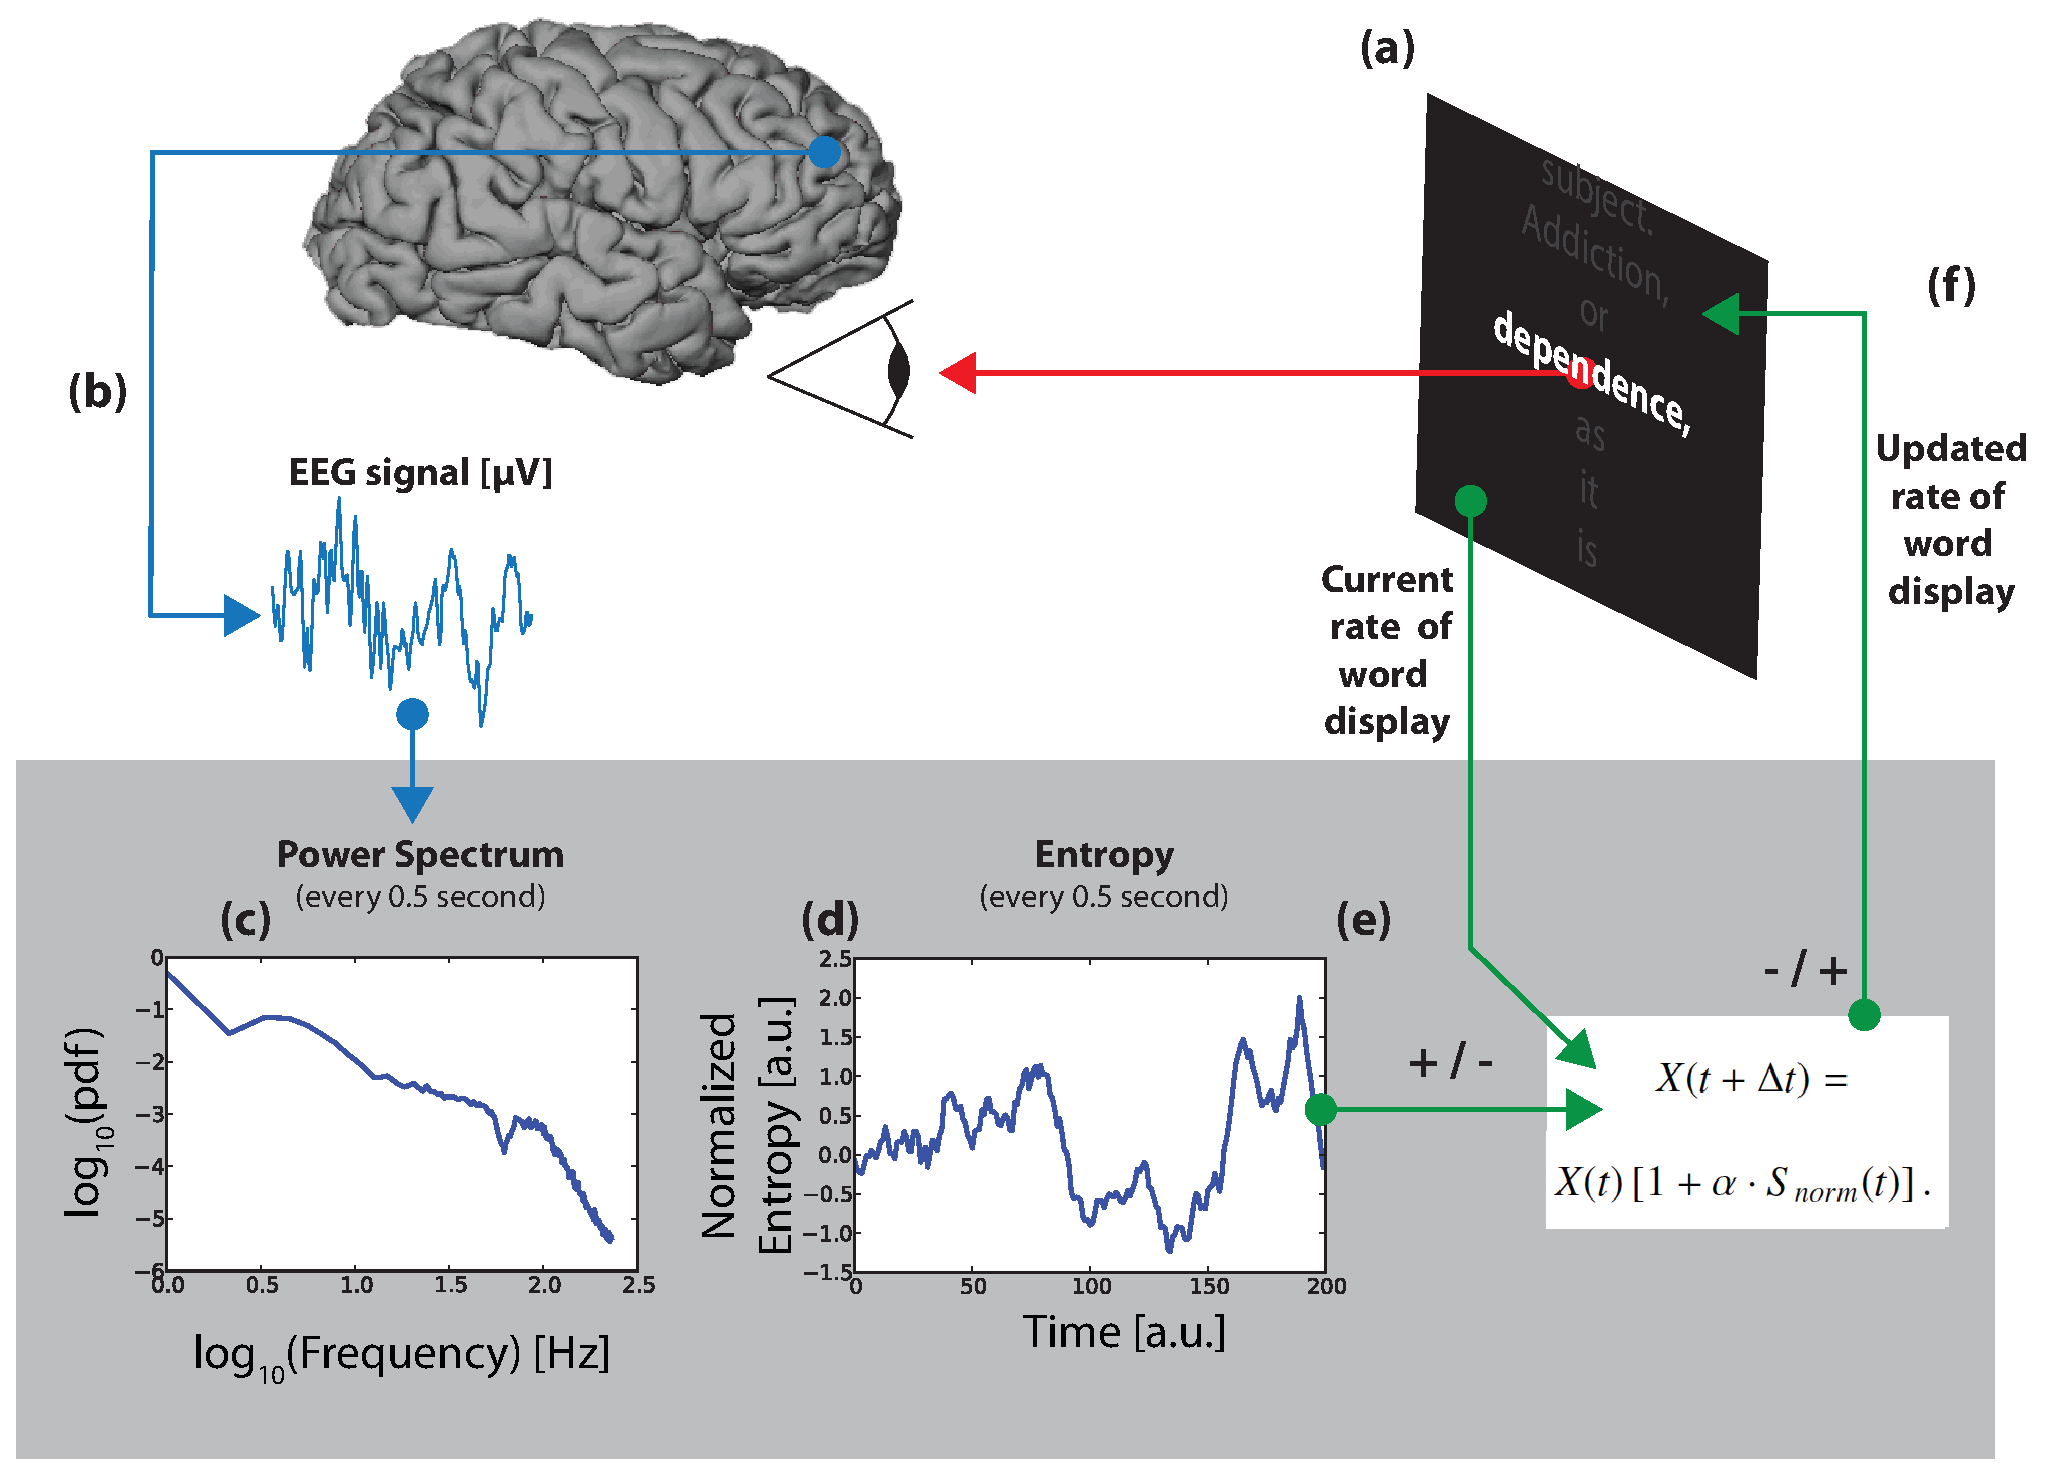
\includegraphics[width=14cm]{../figures2/apparatus.eps}
\caption{Brain speed-reader apparatus: {\bf (a)} Words are displayed and read one after the other at a given rate. {\bf (b)} the EEG signal is recorded through a consumer grade device (here the {\it Neurosky Mindwave}). {\bf (c)} The EEG signal is turned every 0.5 seconds into a power spectrum through a Fourier transform, {\bf (d)} the characteristics of the power spectrum are compressed into a single value characteristic entropy $s$ value. {\bf (e)} A new rate of word display is updated by taking into its current value and $s$. {\bf (f)} The rate of word display is updated accordingly.}
\label{fig:apparatus}
\end{figure}

\begin{figure}[H]
\centering
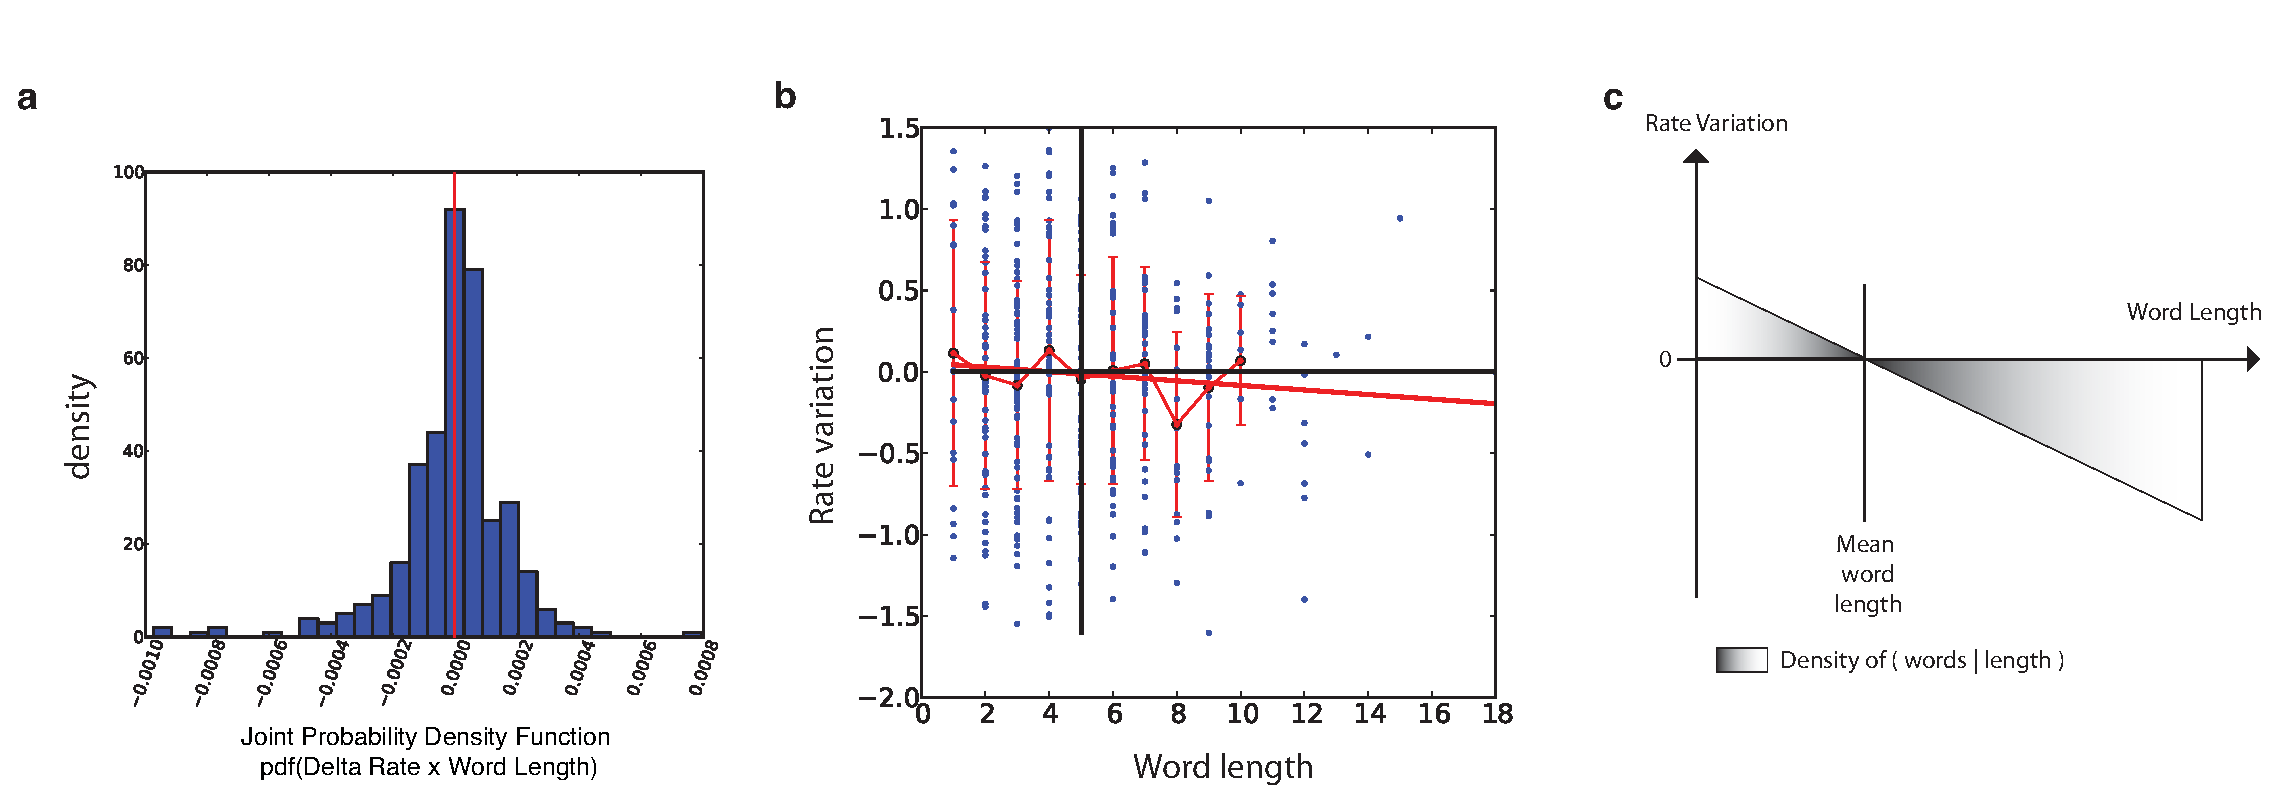
\includegraphics[width=17cm]{../figures2/balance.eps}
\caption{{\bf a.} Joint probability density function pdf(rate change x word length) in the case of a participant capable of controlling the rate of RSVP words presentation. The density function is well-centered around $0$ showing rate change triggered by word long words is counter-balanced by opposite rate change for short words, while average size words trigger little change. {\bf b.} For the same participant, RSVP rate variation as a function of word length. Even though though the plot exhibits large dispersion, one cannot rule out a linear relationship of rate variation as a function of word length, with intercept at the average word length ($\approx 5.1$ characters). {\bf c.} For clarity, schematic representation of the RSVP rate variation as a function of word length, with word length density.}
\label{fig:balance}
\end{figure}

\begin{figure}[H]
\centering
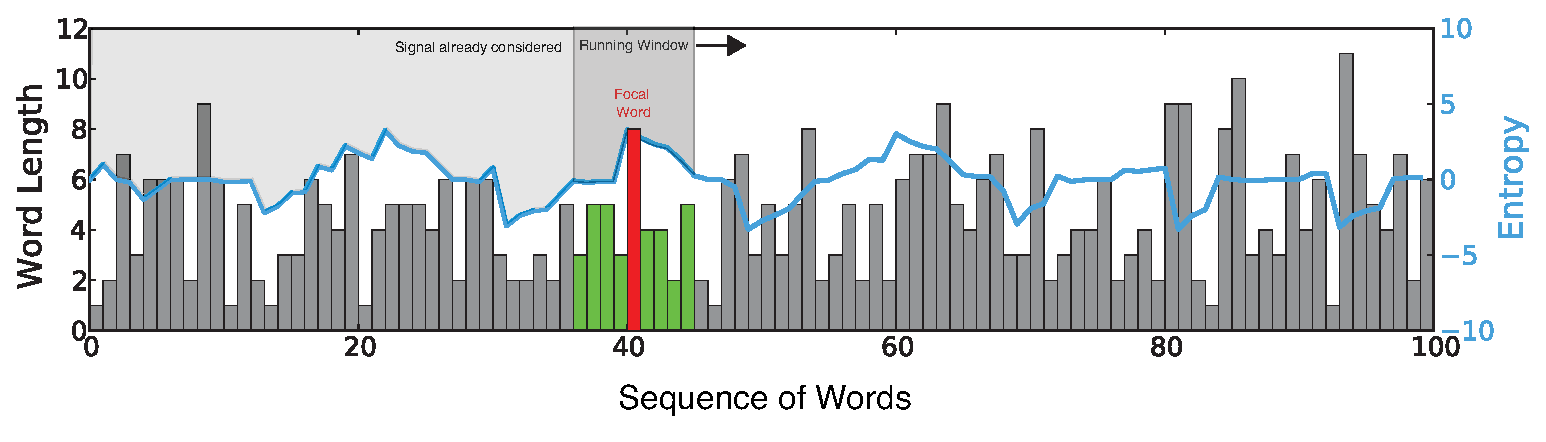
\includegraphics[width=17cm]{Figures/lWordsEntropyTimeline.eps}
\caption{Brain decoding by matching the sequence of word lengths (dark grey bars) and entropy (light blue line). The brain decoding may be performed on the entire sequence, or on the contrary, on the fly, as the text is being read. Brain decoding accuracy increases with the sequence length (i.e., with the number of words in text).}
\label{fig:sequence_decoding}
\end{figure}


%\section{Figures}

\begin{figure}[H]
\centering
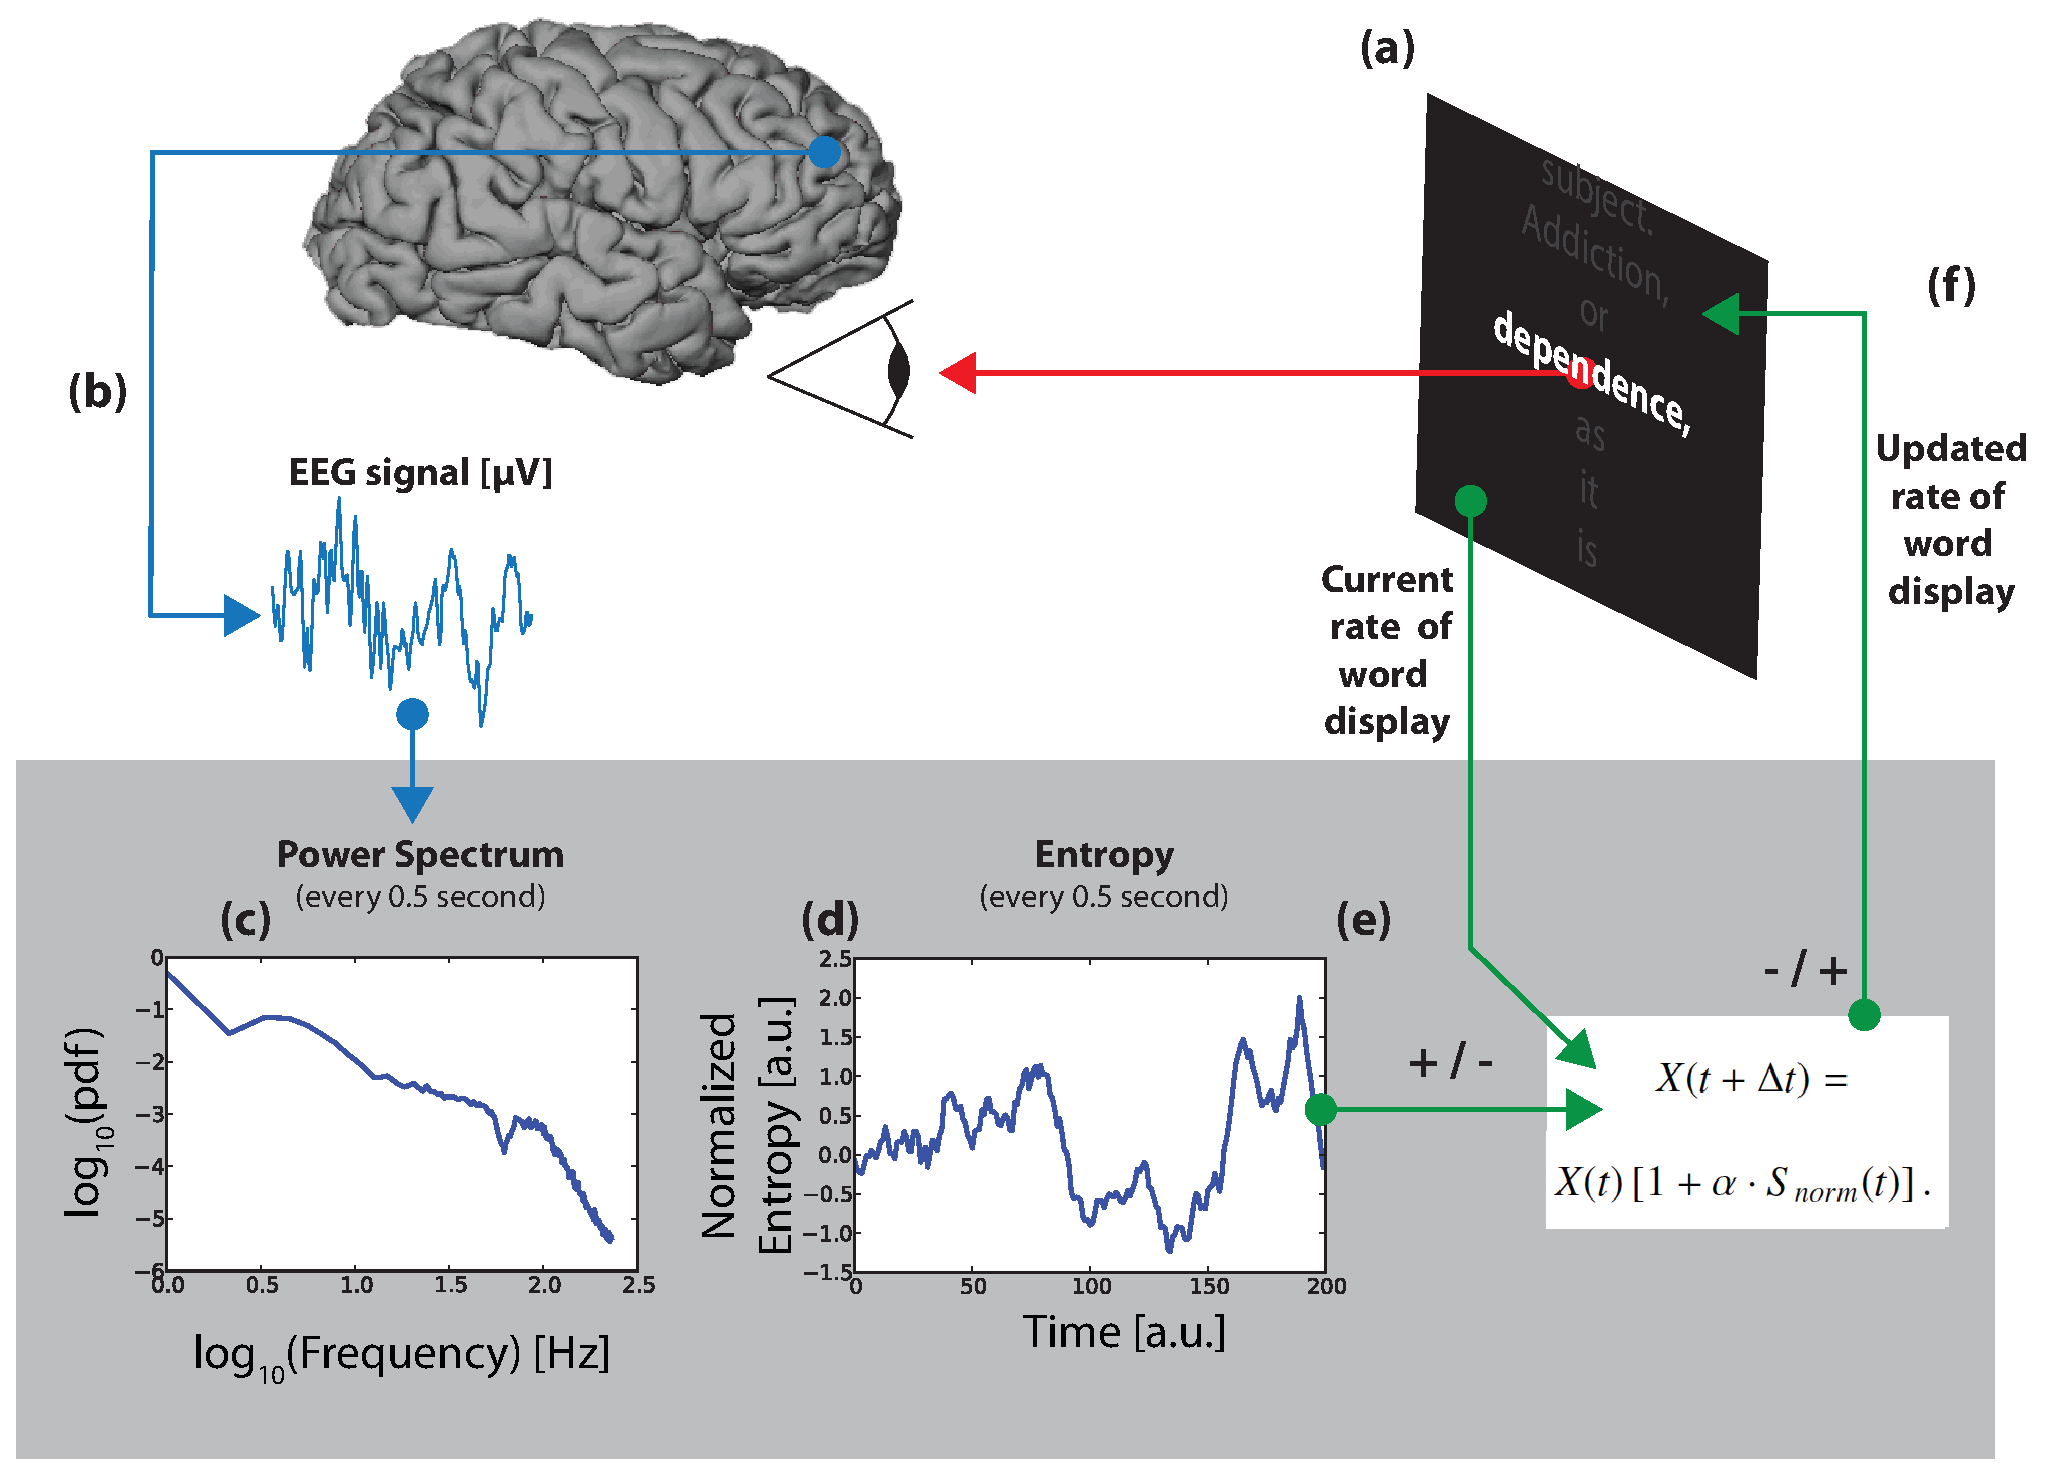
\includegraphics[width=7cm]{../figures2/apparatus.eps}
\caption{Brain speed-reader apparatus: {\bf (a)} Words are displayed and read one after the other at a given rate. {\bf (b)} the EEG signal is recorded through a consumer grade device (here the {\it Neurosky Mindwave}). {\bf (c)} The EEG signal is turned every 0.5 seconds into a power spectrum through a Fourier transform, {\bf (d)} the characteristics of the power spectrum are compressed into a single value characteristic entropy $s$ value. {\bf (e)} A new rate of word display is updated by taking into its current value and $s$. {\bf (f)} The rate of word display is updated accordingly.}
\label{fig:apparatus}
\end{figure}

\begin{figure}[H]
\centering
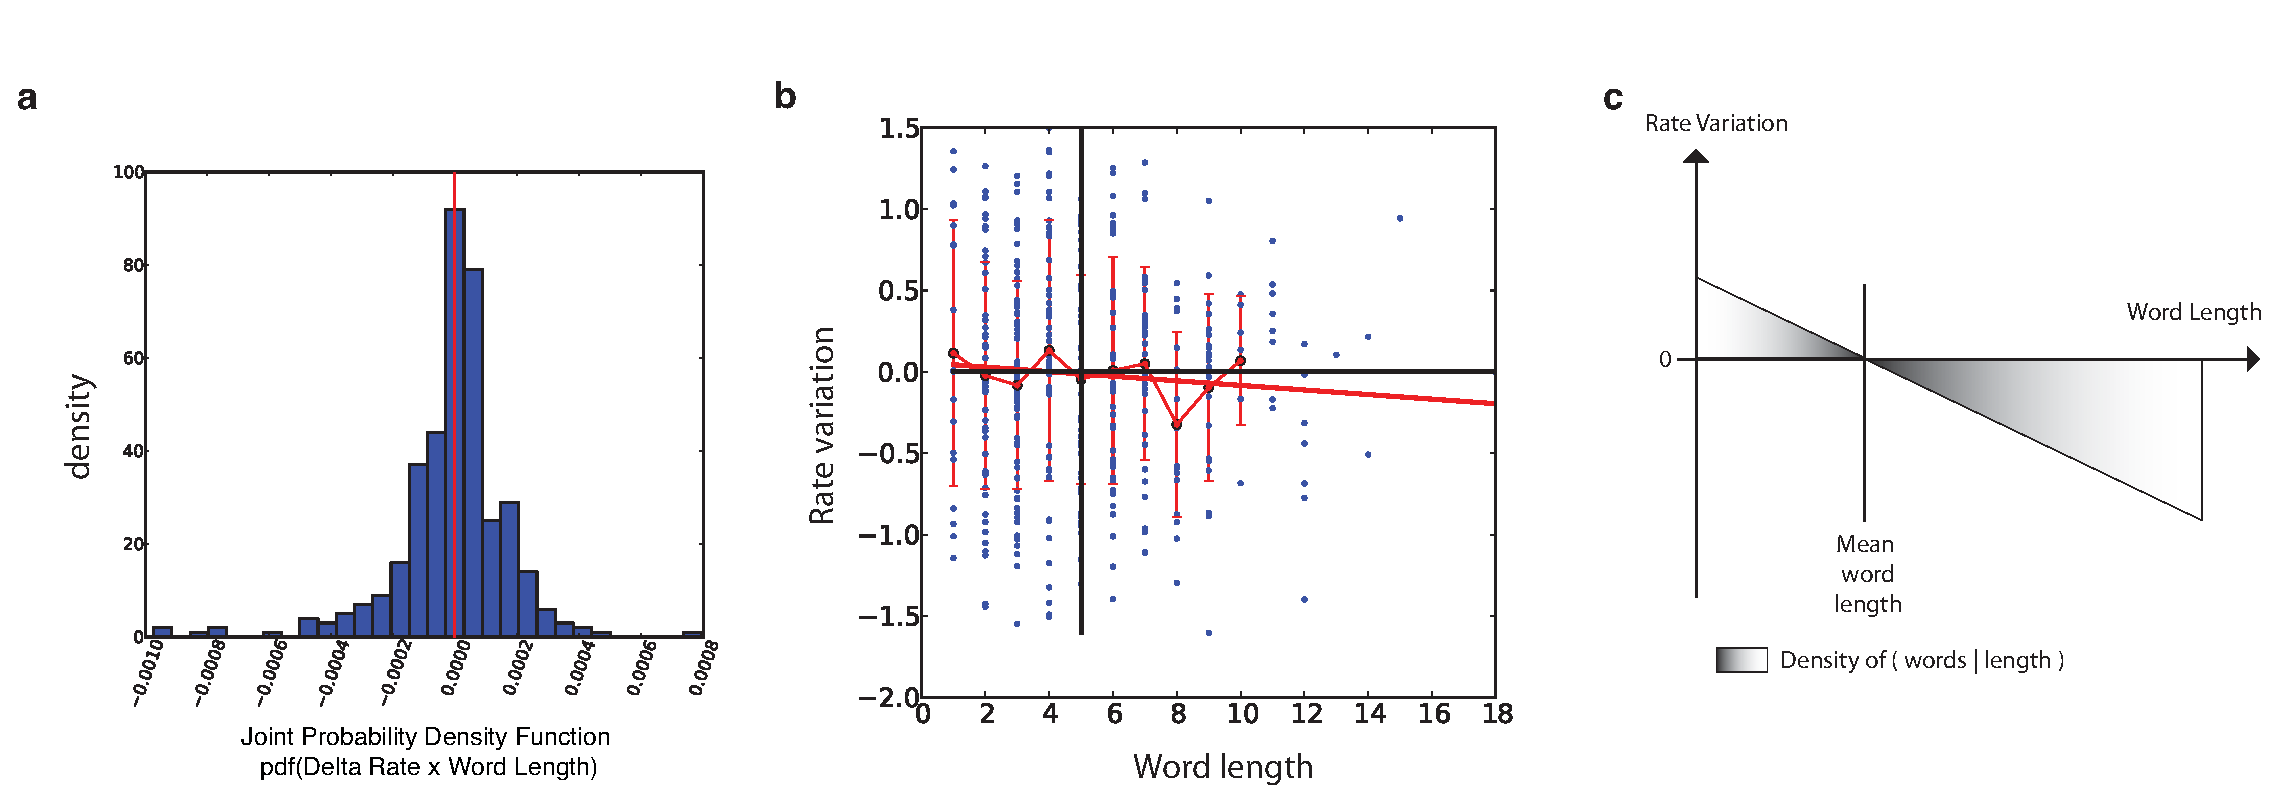
\includegraphics[width=17cm]{../figures2/balance.eps}
\caption{{\bf a.} Schematic representation of the balance of rate change $\Delta_{rate}$ as a function of word length $l_{words}$. The color gradient shows schematically the word density conditioned on their length. This is the canonical or most desirable situation: Around the mean word length the deterministic component of $\Delta_{rate}$ is close to zero. For words with length smaller, the deterministic part of the rate increases, while for words with length larger than the mean, the rate is decreased. The dotted line shows another possible configuration, with acceleration occurring when words are longer. Empirical evidence for the latter case is shown  in Figure \ref{fig:examples} for some typical successful and failed attempts to maintain a balance. ({\bf c}) The joint probability density function $pdf( \Delta_{rate} \times l_{words})$ is well balanced, yet skewed, showing that good control is achieved, along with a good capacity to change the rate of word display.}
\label{fig:apparatus}
\end{figure}

%The linear regression of the average $\Delta_{rates}$ for each word length (for $l_{words} < 10$) exhibits a slope $= 4(1)\times10^{-3}$ ($p < 0.01$). The intersection of $l_{words}(\Delta_{rates} =0) = 4.43$ very close to the average word length (in the text). The error bars show the dispersion (standard deviation of  $\Delta_{rates}$ for each word length. This dispersion is rather large reflecting the stochastic nature of complex brain activation sand the coarse measure obtained from the single electrode EEG headset.

\begin{figure}[H]
\centering
\includegraphics[width=12cm]{../figures2/examples.eps}
\caption{Four examples of successful and failed neuro-feedback control strategies. For each case, three panels are shown (from left to right): (i) Evolution of rate at each displayed word, (ii) rate change as a function of word length at each time step, and (iii)  rate change in the vicinity of large words (9 or more characters, red line), versus words with smaller than 5 characters (blue). The 90\% confidence intervals (light blue area) are obtained by replacement bootstrapping (100 samples of same size as large words are randomly drawn from small words). {\bf a.} Illustration of a very well controlled RSVP, with a sharp and localized drop of word presentation rate around the time large word occurrence. {\bf b.} Opposite strategy with rate increased around large words. {\bf c.} Yet another neuro-feedback strategy with the rate being controlled after the word has occurred. {\bf d.} Failed strategy: Compared to {\bf a}, {\bf b} and {\bf c} the rate change is consistently negative, hence dragging RSVP towards the lower rate limit. Note also in {\bf c} how the rate change as a function of word length (middle panel) is unbalanced around the 0-rate change (horizontal black line) and the mean word length (vertical black line), on the  contrary to {\bf a}, {\bf b} and {\bf c}.}
\label{fig:examples}
\end{figure}


\begin{figure}[H]
\centering
%\includegraphics[width=12cm]{../figures2/examples.eps}
\caption{Here a figure on how the rate is influenced by the power septrum. The idea is to cherry pick moments of high rate change, and look how the power spectrum (and entropy) influences these changes (keep in mind the smoothing, which should reduce the effects of pSpectrum changes on the rate.).}
\label{fig:S_vs_rate}
\end{figure}

\begin{figure}[H]
\centering
%\includegraphics[width=12cm]{../figures2/examples.eps}
\caption{To measure whether there is an effect in the constant rate case, one must first reverse engineer how the rate influences some power spectrum, and how it influences the rate}
\label{fig:constant_rate}
\end{figure}





%\setcounter{section}{0}
%\renewcommand\thesection{\Alph{section}}
%\renewcommand\thesubsection{\thesection.\arabic{subsection}}
%\renewcommand\thesubsubsection{\alph{subsubsection}}
%\clearpage
%\begin{center}
%{\bf \Huge Supplementary Materials}
%\end{center}
%\vspace{2cm}


%\section*{Tables}
%\begin{table}[!ht]
%\caption{
%\bf{Table title}}
%\begin{tabular}{|c|c|c|}
%table information
%\end{tabular}
%\begin{flushleft}Table caption
%\end{flushleft}
%\label{tab:label}
% \end{table}

\end{document}

